\chapter{Comparative Study of Language Embedding Models}
\section{Introduction}
In this chapter, we evaluate the performance of the various embedding models discussed in \secref{sec:emb} in predicting the compositionality of MWEs; specifically English binary noun compounds (NN) and adjective-noun pairs (ADJ-N). Our results show that \wordtovec performs the best, followed by \fasttext and \infersent. We discover, surprisingly, that recently-proposed contextualised embedding models such as \bert and \elmo do not perform impressively in this task. We also experiment with using paraphrases to aid prediction and obtain promising results.

\section{Datasets}
\label{sec:datasets}
We use four datasets for our experiments and evaluate each model's performance using Pearson's correlation coefficient ($r$) to compare the similarity scores obtained with the annotated compositionality scores provided.

\paragraph{\reddy}
The dataset of \cite{Reddy2011} contains 90 English binary noun compounds, along with human-annotated scores of their overall compositionality and component-specific compositionality, ranging from 0 (completely non-compositional) to 5 (completely compositional). 30 annotators worked over Amazon Mechanical Turk to select the definition of the compound noun that occured most frequently in the 5 example sentences provided and score the compound for literality based on the most frequent definition. The final compositionality scores were the average of the annotations with Spearman's $\rho$ greater than 0.6, as well as other annotions that were within the range of $\pm$1.5 from the task's mean.

\noindent
For our experiments, we consider the overall compositionality scores only.

\paragraph{\ramisch}
Similar to \reddy, the English dataset of \cite{Ramisch2016} contains 90 binary noun compounds with annotated scores of compositionality ranging from 0 to 5, both overall and component-specific. It also contains a list of paraphrases for each NC, presented in decreasing order of popularity among the annotators. The scores were derived from 15 human intelligence tasks, wherein annotators were made to perform 5 subtasks for each compound noun:
\begin{enumerate}
    \item Read the noun compound itself
    \item Read 3 sentences containing the compound noun
    \item Provide 2-3 paraphrases for the noun compound based on its meaning as seen in the sentences
    \item Provide a judgement score from 0-5 using a Likert scale of how much of the meaning of the compound comes from the modifier and head separately
    \item Provide a judgement score from 0-5 using a Likert scale of how much the meaning of the compound comes from its components overall
\end{enumerate}
The final scores provided are an average of the annotations.

\noindent
We use only the overall compositionality scores and the paraphrase data in our work.
\paragraph{\discoj}
The English dataset from the DiSCo shared task \citep{Disco2011} contains a total of 348 binary compounds, comprising adjective--noun, verb--noun\textsubscript{subj} and verb--noun\textsubscript{obj} pairs, along with their overall compositionality rating ranging from 0 to 100. The phrases were extracted semi-automatically and their relations were assigned by patterns and checked manually. The compositionality scores were collected from Amazon Mechanical Turk, where workers were presented with 4-5 randomly sampled sentences from the UK English WACKy corpora. The standard number of judgments per target phrase was 20. The final scores were computed by averaging over all the judgements per phrase.

\noindent
We focus on the 145 adjective--noun pairs in this study.
\paragraph{\farahm}
This dataset comprises 1042 English binary noun compounds with four accompanying compositionality labels of either 0 or 1. The four human experts were asked to label the pair 0 for compositional and 1 for non-compositional. Unlike the previous datasets, \farahm presents a binary classification task \citep{Farah2015c}. In addition to compositionality labels, each noun compound also has four conventionalization labels of either 0 (unconventional) or 1 (conventional). 

\noindent
For our experiments, we compute the average of the four labels to produce a score ranging from [0,1] to match our regression task. \figref{fig:datasets} shows a section of the datasets used in this study.
\begin{figure*}[h!]
\centering
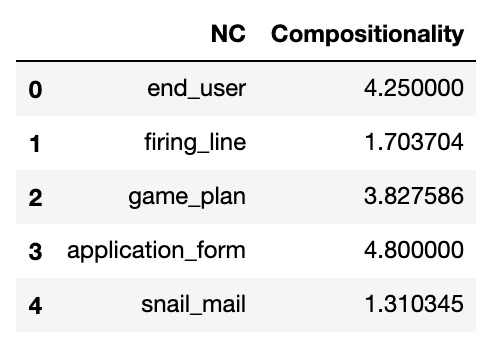
\includegraphics[width = .32\textwidth,]{Figures/reddy.PNG}
\small (a) \reddy
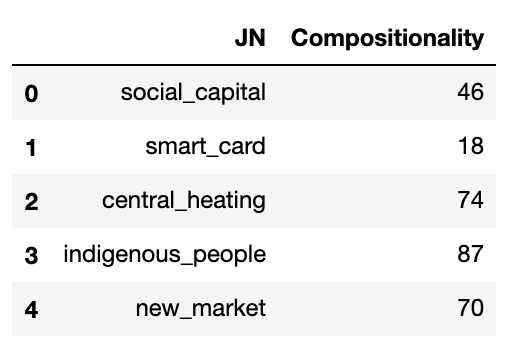
\includegraphics[width = .33\textwidth]{Figures/disco_j.PNG}
\small (b) \discoj
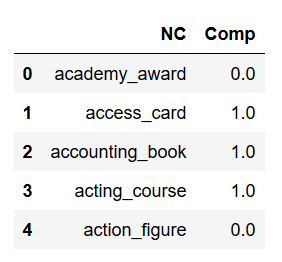
\includegraphics[width = .25\textwidth]{Figures/farahm_after.PNG}
\small (c) \farahm
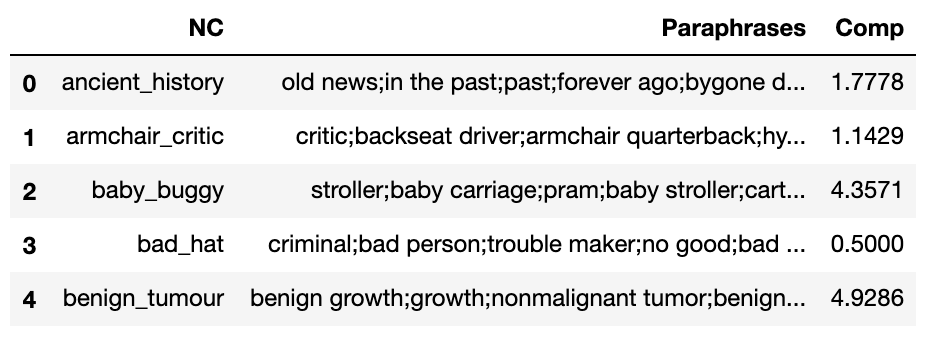
\includegraphics[width = .7\textwidth]{Figures/ramisch.PNG}
\small (d) \ramisch
\caption{Datasets used in this study}
\label{fig:datasets}
\end{figure*}

\begin{table}[t]
\begin{center}
\begin{tabular}{lSS@{\,}l}
  \toprule
  Dataset & $\mu$ & $\sigma$ \\
  \midrule
  \reddy & 53.2 & 30.0 \\
  \ramisch & 52.6 & 35.0 \\
  \discoj & 68.1 & 21.7 \\
  \farahm &  83.1 & 31.8 \\
  \midrule
  Overall & 64.25 & 29.6 \\
\bottomrule
\end{tabular}
\caption{Mean ($\mu$) and standard deviation ($\sigma$) of the compositionality scores of the datasets, over a normalised range $[0,100]$.}
\label{tab:stats}
\end{center}
\end{table}

\bigskip
\noindent
The summary of compositionality scores across the three datasets in \tabref{tab:stats} indicates there is a reasonable distribution of data in terms of compositionality, with \reddy and \ramisch being roughly comparable and covering a broad (and somewhat balanced) spectrum of compositionalities, while \discoj is more skewed towards compositional usages, with lower standard deviation. \farahm's mean shows us it has a higher distribution of compositional noun compounds.

Although we conduct our experiments on English datasets, they can be applied to other languages as we do not perform any kind of language-specific manipulation of the data.

\section{Methodology}
\label{sec:method}
We compute the overall compositionality of an MWE using three broad metrics-- direct composition, paraphrase similarity, and a combined metric. In all experiments, the similarity of a pair of vectors is measured using cosine similarity.

\subsection{Direct Combination}
\label{sec:direct}
Intuitively, an MWE appearing in similar contexts to its component words is likely to be compositional. Following \cite{Salehi2015} and \cite{Reddy2011}, we compare the vector representation of an MWE with that of its component words directly in one of two ways:
\begin{enumerate}
    \item We perform an element-wise sum to obtain a `combined' vector, which is then compared with the vector of the MWE
    \begin{eqnarray}
    \presum =  \cos(\MWEvec, \MWEonevec + \MWEtwovec)
\end{eqnarray}
    \item We combine the scores obtained by individually comparing the vector of the MWE with that of its components post-hoc, via a weighted sum
    \begin{eqnarray}
    \postsum = & \alpha \cos(\MWEvec, \MWEonevec) +  
     (1 - \alpha) \cos(\MWEvec, \MWEtwovec)
    \end{eqnarray}
\end{enumerate}

Here, \MWEvec, \MWEonevec, and \MWEtwovec are the embeddings for the combined MWE, first component and second component, respectively. $\MWEonevec + \MWEtwovec$ is the element-wise sum of the vectors of each of the component words of the MWE; and $\alpha \in [0,1]$ is a scalar which allows us to vary the weight of the respective components in predicting the compositionality of the compound. This helps us effectively capture the compositionality of the MWE with regards to each of its individual constituents. We do not perform any tuning of $\alpha$ over held-out data and are, as such, overfitting as we select the best-performing $\alpha$ post hoc. We do, however, present analysis of hyper-parameter sensitivity in \secref{sec:results}.

It is noteworthy that while all methods are presented and evaluated in terms of two-element MWEs in this work, they are trivially generalisable to multi-element MWEs.

\subsection{Paraphrase Similarity}
Another intuition is that a compositional MWE would appear in similar contexts to the component words of its paraphrases, since each paraphrase provides an interpretation of its semantics (for e.g. the paraphrases \textit{``old times''} and \textit{``long long ago''} offer a rough explanation of the meaning of the MWE \textit{``ancient history''}). The \ramisch dataset (described in \secref{sec:datasets}) provides one or more paraphrases for each MWE. We calculate the similarity of the embeddings of the MWE and its paraphrases using three formulae:
\begin{eqnarray}
\firstpara = & \cos(\MWEvec, \paravec[1])\\
\avgparapre = & \cos(\MWEvec, \sum_i \paravec[i])\\
\avgparapost = & \frac{1}{N} \sum_{i=1}^N \cos(\MWEvec, \paravec[i])
\end{eqnarray}
where \paravec[1] and \paravec[i] denote the embeddings of the first (most popular) and $i$-th paraphrases, respectively.

In the case of \avgparapost, we considered computing the maximum instead of the average (as we report here) of the similarity scores between each paraphrase and its MWE, following the intuition that an MWE would be similar to at least one reported paraphrase, rather than all of them. However, the results for the average similarity were empirically higher across models.
\subsection{Combined Metric}
Finally, we combine the results obtained from the aforementioned methods:
\begin{eqnarray}
  \begin{split}
    \combined = & \beta\max(\presum, \postsum) + \\
    & (1 - \beta)\max(\firstpara, \avgparapre, \avgparapost) \\
  \end{split}
\end{eqnarray}
$\beta\in[0,1]$ is a scalar weighting factor used to balance the effects of the two methods, in order to measure the extent to which the compositionality is determined by each of the methods. We use the $\max$ operator here to combine the sub-methods for each of the direct composition and paraphrase methods since all methods tend to underestimate the compositionality. It was also empirically found to be superior to taking the mean.

\section{Experiments}
We implement the metrics detailed above using each of the language embedding models discussed in \secref{sec:emb} and compare their performance. Where available, we made use of pretrained models as is standard practice in NLP. As the different models are trained on different corpora, we are not attempting to perform a controlled comparative evaluation of the different models, so much as a comparison of the standard pretrained versions of each. If we were to retrain our own models over a standard dataset, such as English Wikipedia\textsuperscript{\ref{wiki}}, we would expect the results for the document-level embedding models in particular to drop.

\paragraph{\wordtovec} \wordtovec is a word-level embedding model. Therefore, if fed with one of our MWEs, it will perform delimiting by space and generate embeddings for each of its component words instead. To circumvent this, we would like to treat the MWE as a single word (spaces removed) and generate a single representative vector embedding. For instance, we would generate an embedding for \textit{``closeshave''} to represent the MWE \textit{``close shave''}. However, another issue with \wordtovec is that it is incapable of handling out-of-vocabulary words (OOVs) and, hence, would fail to generate a representation for \textit{``closeshave''} if it has never seen it before (which is understandable, given all occurrences of the MWE in the training corpus would include the space). The solution then is to remove the space from all occurrences of the MWEs in the training corpus.

We trained the gensim implementation of \wordtovec on a recent English Wikipedia dump,\footnote{\label{wiki}Dated 07-Jan-2019} after pre-processing it (removing the formatting and punctuation) and, following \cite{Salehi2015}, concatenating each occurence of the MWE in our datasets (i.e., every occurence of \textit{``close shave''} in the corpus becomes \textit{``closeshave''}), making an over-optimistic assumption that every occurring collocation of the component words represent the MWE in question. The resultant \wordtovec model generates vector representations with 300 dimensions using SkipGram and a minimum count and window size of 5.

In cases where the model fails to generate an embedding for the expression due to low token frequency, and we observe 2, 8 and 25 cases of this in \reddy, \ramisch and \discoj, respectively, we assign a default compositionality score of 0.5 (neutral; based on a range of [0,1]). For paraphrases, we compute an element-wise sum of the embeddings for each of the component words to serve as the embedding of the phrase. We do this because token-level identification of each paraphrase in the training corpus is not feasible and the element-wise sum approach is consistent with the MWE compositionality prediction approaches of \cite{Salehi2015} and \cite{Reddy2011} and a paraphrase could be thought of as an MWE in its own right.

\paragraph{\fasttext}
Since \fasttext represents each word as a bag of its ngrams, it is capable of generating embeddings for OOV terms as well. Therefore, no manipulation of the training corpus is necessary. However, like \wordtovec, it performs whitespace delimiting and we therefore need to preprocess our MWEs and paraphrases the same way as stated above to derive a \textit{fused compound} (i.e. we use the embedding for \textit{``closeshave''} to represent \textit{``close shave''}).

We used the 300-dimensional \fasttext model pre-trained on Common Crawl and Wikipedia using CBOW (\fasttextpre), as well as one trained over our Wikipedia corpus\textsuperscript{\ref{wiki}} using skip-gram (\fasttext).

\paragraph{\doctovec}
Since \doctovec is a document-level embedding, we treat the MWE as a two-word document, as well as each of its components as single word documents to generate their embeddings.

We used the gensim implementation of \doctovec pretrained on Wikipedia data using the \wordtovec skip-gram models pretrained on Wikipedia and AP News.\footnote{\url{https://github.com/jhlau/doc2vec}}

\paragraph{\infersent}
Similar to the approach used in \doctovec, we treat the MWE as a two-word sentence and its components as single word sentences to generate their embeddings using \infersent, which is a sentence-level embedding.

We used two pretrained versions of \infersent: \infersent[\glove] and \infersent[\fasttext]. Each generates a representation of 4096 dimensions, trained over the 1,000,000 most popular English words using \glove \citep{Jeffrey2014} and \fasttext, respectively.

\paragraph{Contextualised Embeddings}
We used the pretrained implementations of \elmo, \bert and \flair available in the \flair framework.\footnote{\url{https://github.com/zalandoresearch/flair}}

We used sentences extracted from the Brown corpus where available in order to derive contextualised interpretations. We used literary context as it was more likely to have instances of the more idiomatic or non-compositional MWEs, as opposed to news or Wikipedia corpora. We extracted 25 sentences at random for each MWE, except where there were fewer sentences in the corpus.

We also included a naive context-independent implementation of \elmo, \bert and \flair in our study, consistent with the other models. This also helped us test our intuition that the relative compositionality of even novel compounds could potentially be predicted from its component words alone. Consider for instance the unseen expression \textit{``giraffe potato''}, which could have the plausible compositional interpretation of a potato shaped like a giraffe (considering contexts like \textit{round potato}, say), while \textit{``couch intelligence''} might have no natural interpretation given its context and could, therefore, be assumed to have a non-compositional meaning.

%Nav: clean up diagrams and tables, rewrite the section to include insights on farahm dataset also
\section{Results and Discussion}
\label{sec:results}
The results from our experiments on the \reddy,  \discoj, \farahm and \ramisch datasets can be found in \tabref[s]{tab:reddy},\ref{tab:discoj}, \ref{tab:farahm} and \ref{tab:ramisch}, respectively, with the best performing $\alpha$s and $\beta$s mentioned for each embedding model.

\begin{table}[t]
\minipage{0.45\textwidth}
\begin{tabular}{lSS@{\,}l}
  \toprule
  Emb.\ method        & {\presum}  & \multicolumn{2}{c}{\postsum} \\
  \midrule
  \wordtovec & \B 0.634 & \B 0.622 & ($\alpha$ = 0.6) \\
  \fasttextpre & 0.223 & 0.285 & ($\alpha$ = 0.3) \\
  \fasttext & 0.217 & 0.287 & ($\alpha$ = 0.3) \\
  \doctovec & -0.049 & 0.025 & ($\alpha$ = 0.0) \\
  \infersent[\glove] & 0.413 & 0.500 & ($\alpha$ = 0.5) \\
  \infersent[\fasttext] & 0.401 & 0.527 & ($\alpha$ = 0.6) \\
  \elmo & 0.339 & 0.406 & ($\alpha$ = 0.5) \\
  \elmocon & 0.363 & 0.406 & ($\alpha$ = 0.5) \\
  \bert & 0.304 & 0.352 & ($\alpha$ = 0.2) \\
  \bertcon & 0.311 & 0.372 & ($\alpha$ = 0.2) \\
  \flair & -0.127 & 0.024 & ($\alpha$ = 0.0) \\
  \flaircon & 0.002 & 0.102 & ($\alpha$ = 0.0) \\
\bottomrule
\end{tabular}
\caption{Pearson correlation coefficient for compositionality prediction results on the \reddy dataset.}
\label{tab:reddy}
\endminipage\hfill
\minipage{0.45\textwidth}
\begin{tabular}{lSS@{\,}l}
  \toprule
  Emb.\ method        & {\presum}  & \multicolumn{2}{c}{\postsum} \\
  \midrule
  \wordtovec & \B 0.427 & \B 0.419 & ($\alpha$ = 0.4) \\
  \fasttextpre & 0.339 & 0.353 & ($\alpha$ = 0.6) \\
  \fasttext & 0.374 & 0.419 & ($\alpha$ = 0.4) \\
  \doctovec & -0.023 & 0.003 & ($\alpha$ = 0.0) \\
  \infersent[\glove] & 0.321 & 0.315 & ($\alpha$ = 0.4) \\
  \infersent[\fasttext] & 0.001 & 0.202 & ($\alpha$ = 1.0) \\
  \elmo & 0.253 & 0.287 & ($\alpha$ = 0.5) \\
  \elmocon & 0.282 & 0.316 & ($\alpha$ = 0.5) \\
  \bert & 0.154 & 0.177 & ($\alpha$ = 0.3) \\
  \bertcon & 0.166 & 0.181 & ($\alpha$ = 0.3) \\
  \flair & 0.261 & 0.291 & ($\alpha$ = 0.4) \\
  \flaircon & 0.272 & 0.303 & ($\alpha$ = 0.4)  \\
\bottomrule
\end{tabular}
\caption{Pearson correlation coefficient for compositionality prediction results on the \discoj[ADJ] dataset.}
\label{tab:discoj}
\endminipage\hfill
\end{table}

\begin{table}[t]
\begin{center}
\begin{tabular}{lSS@{\,}l}
  \toprule
  Emb.\ method        & {\presum}  & \multicolumn{2}{c}{\postsum} \\
  \midrule
  \wordtovec & .244 & \B .35 & ($\alpha$ = 0.9) \\
  \fasttextpre & .197 & .291 & ($\alpha$ = 0.8) \\
  \fasttext & .203 & .295 & ($\alpha$ = 0.8) \\
  \doctovec & .083 & .088 & ($\alpha$ = 0.8) \\
  \infersent[\glove] & .002 & .010 & ($\alpha$ = 1.0) \\
  \infersent[\fasttext] & -.059 & .019 & ($\alpha$ = 1.0) \\
  \elmo & \B.283 & .278 & ($\alpha$ = 0.5) \\
  \elmocon & .291 & .280 & ($\alpha$ = 0.5) \\
  \bert & .176 & .193 & ($\alpha$ = 0.9) \\
  \bertcon & .179 & .191 & ($\alpha$ = 0.9) \\
  \flair & .222 & .23 & ($\alpha$ = 0.6) \\
  \flaircon & .229 & .247 & ($\alpha$ = 0.6) \\
\bottomrule
\end{tabular}
\caption{Pearson correlation coefficient for compositionality prediction results on the \farahm dataset.}
\label{tab:farahm}
\end{center}
\end{table}

\begin{table*}[t!]
\begin{center}
\begin{tabular}{lSS@{\,}lSSSS@{\,}l}
\toprule
  Emb.\ method        & {\presum}  & \multicolumn{2}{c}{\postsum} & {\firstpara} & {\avgparapre} & {\avgparapost} & \multicolumn{2}{c}{\combined} \\
  \midrule
  \wordtovec & \B 0.581 & \B 0.571 & ($\alpha$ = 0.6) & 0.443 & 0.510 & 0.504 & 0.677 & ($\beta$ = 0.9) \\
  \fasttextpre & 0.395 & 0.446 & ($\alpha$ = 0.7) & 0.242 & 0.531 & 0.703 & 0.703 & ($\beta$ = 0.0) \\
  \fasttext & 0.464 & 0.532 & ($\alpha$ = 0.7) & 0.548 & 0.613 & 0.673 & 0.673 & ($\beta$ = 0.0) \\
   \doctovec & -0.157 & 0.039 & ($\alpha$ = 1.0) & 0.388 & 0.334 & 0.373 & 0.419 & ($\beta$ = 0.3) \\
   \infersent[\glove] & 0.321 & 0.427 & ($\alpha$ = 0.7) & \B 0.636 & 0.700 & \B 0.741 & \B 0.783 & ($\beta$ = 0.5) \\
  \infersent[\fasttext] & 0.169 & 0.221 & ($\alpha$ = 0.6) & 0.488 & \B 0.712 & 0.636 & 0.712 & ($\beta$ = 0.0) \\
  \elmo & 0.420 & 0.459 & ($\alpha$ = 0.6) & 0.361 & 0.488 & 0.546 & 0.546 & ($\beta$ = 0.2) \\
  \elmocon & 0.448 & 0.486 & ($\alpha$ = 0.6) & 0.366 & 0.486 & 0.550 & 0.621 & ($\beta$ = 0.2) \\
  \bert & 0.071 & 0.086 & ($\alpha$ = 1.0) & 0.242 & 0.531 & 0.583 & 0.583 & ($\beta$ = 0.0) \\
  \bertcon & 0.087 & 0.107 & ($\alpha$ = 1.0) & 0.257 & 0.541 & 0.598 & 0.598 & ($\beta$ = 0.0) \\
  \flair & 0.165 & 0.295 & ($\alpha$ = 0.1) & 0.334 & 0.399 & 0.492 & 0.492 & ($\beta$ = 0.0) \\
  \flaircon & 0.177 & 0.311 & ($\alpha$ = 0.1) & 0.344 & 0.409 & 0.512 & 0.512 & ($\beta$ = 0.0) \\
  \bottomrule
\end{tabular}
\caption{Pearson correlation coefficient for compositionality prediction results on the \ramisch dataset.}
\label{tab:ramisch}
\end{center}
\end{table*}

\pgfplotsset{width=16cm,height=10cm}
\begin{figure}[h!]
\begin{center}
\begin{tikzpicture}
\begin{axis}[
    bar width=2mm,
    ybar,
    %enlargelimits=0.15,
    legend style={at={(0.5,-0.25)},
      anchor=north,legend columns=-1},
    ylabel={$r$},
    symbolic x coords={doc2vec, Infersent, fastText,ELMo,BERT, Flair, word2vec},
    xtick=data,
    xticklabel style = {rotate=10},
    ymajorgrids=true,
    %nodes near coords,
    %nodes near coords align={vertical},
    ]
\addplot[draw=blue!40,fill=blue!20] table[x=x,y=farahm] \datasetq;
\addplot[draw=red!40,fill=red!40] table[x=x,y=ramisch] \datasetq;
\addplot[draw=orange!40,fill=orange!40] table[x=x,y=reddy] \datasetq;
\addplot[draw=green!40,fill=green!40] table[x=x,y=discoj] \datasetq;

\legend{\farahm, \ramisch, \reddy, \discoj};
\end{axis}
\end{tikzpicture}
\caption{Overall performance -- Direct Combination}
\end{center}
\end{figure}

\begin{figure}[t]
\begin{center}
\pgfplotsset{width=16cm,height=10cm}
\begin{tikzpicture}
\begin{axis}[
    bar width=2mm,
    ybar,
    %enlargelimits=0.15,
    legend style={at={(0.5,-0.25)},
      anchor=north,legend columns=-1},
    ylabel={$r$},
    symbolic x coords={doc2vec, Infersent, fastText,ELMo,BERT, Flair, word2vec},
    xtick=data,
    xticklabel style = {rotate=10},
    ymajorgrids=true,
    %nodes near coords,
    %nodes near coords align={vertical},
    ]
\addplot[draw=red!40,fill=red!40] table[x=x,y=direct] \datasetp;
\addplot[draw=orange!40,fill=orange!40] table[x=x,y=para] \datasetp;
\addplot[draw=blue!40,fill=blue!40] table[x=x,y=combined] \datasetp;

\legend{Direct Combination, Paraphrases, Combined};
\end{axis}
\end{tikzpicture}
\caption{Use of Paraphrases (\ramisch)}
\end{center}
\end{figure}

\begin{figure*}[t!]
    \centering
        \begin{tikzpicture}
\begin{axis}[
axis lines=middle,
width=0.5*\textwidth,
height=3in,
ymax=1.0,
ymin=-0.2,
xmin=0.0,
xmax=1.0,
  axis x line = bottom,
    x label style={at={(axis description cs:0.5,-0.1)},anchor=north},
    y label style={at={(axis description cs:-0.1,.5)},rotate=90,anchor=south},
    xlabel= $\alpha$,
  ylabel=$r$,
  xticklabel style = {rotate=30,anchor=east},
   enlargelimits = false,
  xticklabels from table={alpha_reddy.dat}{X},xtick=data]
\addplot[orange,thick] table [y=elmo,x=X]{alpha_reddy.dat};
\addplot[green,thick] table [y= fasttext,x=X]{alpha_reddy.dat};
\addplot[blue,thick] table [y= d2v,x=X]{alpha_reddy.dat};
\addplot[brown,thick] table [y= is1,x=X]{alpha_reddy.dat};
\addplot[red,thick] table [y= is2,x=X]{alpha_reddy.dat};
\addplot[yellow,thick] table [y= w2v,x=X]{alpha_reddy.dat};
\addplot[purple,thick] table [y= bert,x=X]{alpha_reddy.dat};
\addplot[pink,thick] table [y= flair,x=X]{alpha_reddy.dat};
\end{axis}
\end{tikzpicture}
        \begin{tikzpicture}
\begin{axis}[
  axis lines=middle,
  width=0.5*\textwidth,
  height=3in,
  ymin=-0.2,
  ymax=1.0,
  xmin=0.0,
  xmax=1.0,
  x label style={at={(axis description cs:0.5,-0.1)},anchor=north},
  y label style={at={(axis description cs:-0.1,.5)},rotate=90,anchor=south},
  xlabel= $\alpha$,
  ylabel=$r$,
  axis x line = bottom,
  legend columns=1, 
  legend pos= outer north east,
  xticklabel style = {rotate=30,anchor=east},
  enlargelimits = false,
  xticklabels from table={alpha_ramisch.dat}{X},xtick=data]
\addplot[orange,thick] table [y=elmo,x=X]{alpha_ramisch.dat};
\addplot[green,thick] table [y= fasttext,x=X]{alpha_ramisch.dat};
\addplot[blue,thick] table [y= d2v,x=X]{alpha_ramisch.dat};
\addplot[brown,thick] table [y= is1,x=X]{alpha_ramisch.dat};
\addplot[red,thick] table [y= is2,x=X]{alpha_ramisch.dat};
\addplot[yellow,thick] table [y= w2v,x=X]{alpha_ramisch.dat};
\addplot[purple,thick] table [y= bert,x=X]{alpha_ramisch.dat};
\addplot[pink,thick] table [y= flair,x=X]{alpha_ramisch.dat};
\end{axis}
\end{tikzpicture}\\
        \begin{tikzpicture}
\begin{axis}[
axis lines=middle,
width=0.5*\textwidth,
height=3in,
ymax=1.0,
ymin=-0.2,
xmax=1.0,
xmin=0.0,
    x label style={at={(axis description cs:0.5,-0.1)},anchor=north},
    y label style={at={(axis description cs:-0.1,.5)},rotate=90,anchor=south},
    xlabel= $\alpha$,
    ylabel=$r$,
  xticklabel style = {rotate=30,anchor=east},
  enlargelimits = false,
  axis x line = bottom,
  xticklabels from table={alpha_discoj.dat}{X},xtick=data]
\addplot[orange,thick] table [y=elmo,x=X]{alpha_discoj.dat};
\addplot[green,thick] table [y= fasttext,x=X]{alpha_discoj.dat};
\addplot[blue,thick] table [y= d2v,x=X]{alpha_discoj.dat};
\addplot[brown,thick] table [y= is1,x=X]{alpha_discoj.dat};
\addplot[red,thick] table [y= is2,x=X]{alpha_discoj.dat};
\addplot[yellow,thick] table [y= w2v,x=X]{alpha_discoj.dat};
\addplot[purple,thick] table [y= bert,x=X]{alpha_discoj.dat};
\addplot[pink,thick] table [y= flair,x=X]{alpha_discoj.dat};
\end{axis}
\end{tikzpicture}
        \begin{tikzpicture}
\begin{axis}[
axis lines=middle,
width=0.5*\textwidth,
height=3in,
ymax=1.0,
ymin=-0.2,
xmin=0.0,
xmax=1.0,
  axis x line = bottom,
    x label style={at={(axis description cs:0.5,-0.1)},anchor=north},
    y label style={at={(axis description cs:-0.1,.5)},rotate=90,anchor=south},
    xlabel= $\alpha$,
  ylabel=$r$,
  xticklabel style = {rotate=30,anchor=east},
   enlargelimits = false,
  xticklabels from table={alpha_farahm.dat}{X},xtick=data]
\addplot[orange,thick] table [y=elmo,x=X]{alpha_farahm.dat};
\addplot[green,thick] table [y= fasttext,x=X]{alpha_farahm.dat};
\addplot[blue,thick] table [y= d2v,x=X]{alpha_farahm.dat};
\addplot[brown,thick] table [y= is1,x=X]{alpha_farahm.dat};
\addplot[red,thick] table [y= is2,x=X]{alpha_farahm.dat};
\addplot[yellow,thick] table [y= w2v,x=X]{alpha_farahm.dat};
\addplot[purple,thick] table [y= bert,x=X]{alpha_farahm.dat};
\addplot[pink,thick] table [y= flair,x=X]{alpha_farahm.dat};
\end{axis}
\end{tikzpicture}
\caption{\farahm}
    \caption{Sensitivity analysis of $\alpha$}
\label{fig:sens}
\end{figure*}

We observe that the $\alpha$s in \tabref[s]{tab:ramisch},\ref{tab:farahm}: are high, implying the compound nouns in \ramisch and \farahm are more compositional in terms of their head (second) nouns. Similarly, the lower $\alpha$ scores in \tabref{tab:reddy} suggest \reddy's compound nouns are more dependent on their modifiers, or first nouns. \tabref{tab:discoj}, on the other hand, shows the $\alpha$s embracing the entire range of $[0,1]$. This suggests the adjective--noun pairs in \discoj display a spread of compositionality. Overall, the methods are sensitive to the choice of the $\alpha$ hyper-parameter, with \elmo and \infersent being particularly sensitive and showing substantial change in output with change in $\alpha$ (\figref[s]{fig:sensReddy},\ref{fig:sensRamisch} and \ref{fig:sensDiscoj}).

We see that for \ramisch (\tabref{tab:ramisch}), \wordtovec achieves the highest scores among the direct combination metrics, while \infersent outperforms the other methods among the paraphrase metrics. We also note that \wordtovec falls behind character embedding models like \fasttext, \elmo and \bert, even when the latter two were performed without context. The lower $\beta$ scores also show the other models favouring the paraphrase approaches, while the high $\beta$ score for \wordtovec shows its preference for direct combination. Overall, we see that the paraphrase metrics provide us with the highest correlation scores, with \infersent garnering scores much higher than \wordtovec's highest score from direct combination.

Our next observation is that, consistent with its performance on \ramisch, \wordtovec performs the best of all models in the direct combination metrics on \reddy and \discoj. Overall, we observe that \wordtovec is consistent in providing the best results based on the metrics outlined in \secref{sec:direct}, while \fasttext and \infersent come a close second and third, respectively, with \fasttext in particular providing substantial correlation scores across metrics (where \infersent and \wordtovec only achieve high scores under a specific metric). It is noteworthy, however, that \wordtovec required explicit modelling of the MWEs during the training step, while the other models did not.

\subsection*{Discussion}
It is not surprising that \infersent, being a document-level embedding model, works better with paraphrase data than the other models. However, \doctovec has really poor scores overall across the three datasets. It does, however, redeem itself with the paraphrases, with substantially higher scores than the direct approach but still quite a way behind the top-scoring methods. 

As mentioned before, we see that the paraphrase metrics achieve much greater results across all models, suggesting this could be a direction for future study (noting the availability requirement for paraphrase data for the MWE in order to apply this method, which has inherent scalability limitations). The combined approach seems to favour the paraphrase results as well, based on the relative $\beta$ values.

One of the reasons \wordtovec did not work as well with the paraphrases could be the naive assumption that \presum is a representation of the paraphrase itself. As we see from the results across the datasets and models, \presum does not entirely capture the compositionality of the MWE, so it is reasonable to assume that a paraphrase would not be accurately represented by  its \presum either. 

\fasttext provides us with impressive scores throughout, and we notice a slight improvement when trained on the same corpus as \wordtovec. However, there is a huge gap in the performance between \wordtovec and \fasttext, especially in the case of \reddy (which could be an issue of a heavier representation of a particular level of compositionality, say).

We also notice that, unlike the noun compounds in \reddy and \ramisch, there is less variance in the relative scores of each method in the case of \discoj[ADJ], with overall results dropping appreciably and the best-performing \wordtovec dropping back in raw $r$ value compared to noun--noun pairs. This suggests that adjective-noun pairs come with inherent nuances of their own that complicate the prediction of their compositionalities and might require further study.

In terms of the contextualised embeddings, we notice that across the three models, there is only a slight increase in correlation when contextual sentences were supplied. This suggests that even with context, these modern embedding techniques are unable to capture non-compositionality as well as their simpler counterparts. 

Further analysis reveals that most models struggle to accurately predict the compositionality of idiomatic noun compounds, as well as semi-compositional terms wherein one of the constituent words are used in a metaphoric sense. In \reddy, for instance, we observe this for \textit{silver bullet} and \textit{snail mail}. Interestingly, while \bert struggles to effectively model compositionality throughout, it is suprisingly the only model able to perfectly predict the compositionality of \textit{snail mail} (which appears as an extreme outlier). This suggests that \bert might be more successful using a different metric. In the case of the adjective-noun phrases in \discoj, we see once more that the models are still unable to accurately predict the compositionality of non-compositional phrases (like \textit{big fish, heavy metal} and \textit{red tape}). This time, however, they are also unable to capture \textit{mobile phone} and \textit{floppy disk}, perhaps because of their relatively archaic use.

\section{Summary}
In this chapter, we investigated the modelling capabilities of various embedding techniques applied to the specific task of predicting the compositionality of MWEs, to see how well they model a mixture of compositionalities in the dataset. Our results indicate that modern character- and document-level embedding methods are inferior to the simple \wordtovec approach proposed by \cite{Salehi2015}. However, the promising results of \fasttext and \infersent across the datasets studied indicate that, among the more modern methods, they are better equipped to handle non-compositionality as they did not require any manipulation of the corpus or knowledge of the MWEs beforehand. We also found that the paraphrase metric results in greater correlation scores across the models.